%!TEX root = main.tex
\section{Evaluation Study Findings\label{sec:eval_findings}}
% \begin{figure*}[t!]
% \minipage{0.6\textwidth}
%   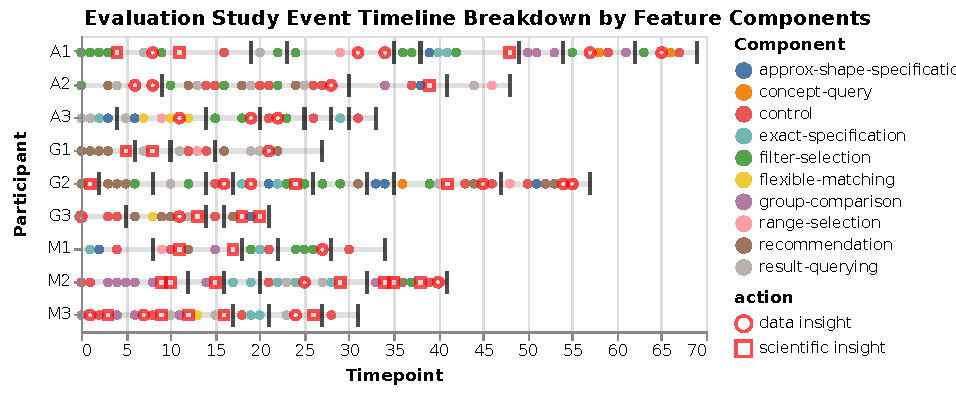
\includegraphics[width=\linewidth]{figures/evalstudytimeline.pdf}
%   \caption{Timeline of event code and component usage, with every timepoint as an event on the x axis. For clarity, we hide most of the event coding labels other than the insight labels. Black vertical tick indicates a session break, signaling the beginning of a new line of inquiry.}\label{fig:evalstudytimeline}
% \endminipage\hfill
% \minipage{0.4\textwidth}
%   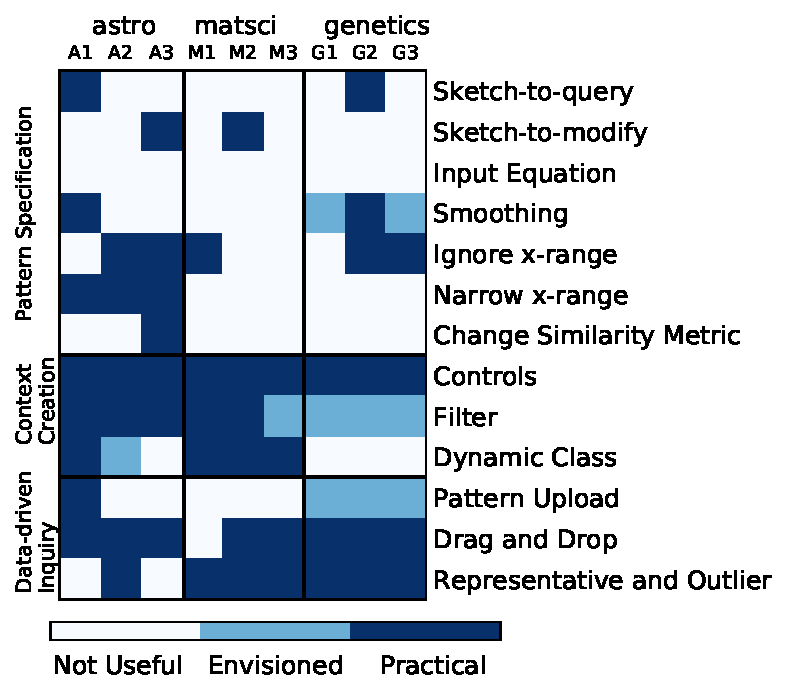
\includegraphics[width=0.8\linewidth]{figures/PENcoding.pdf}
%   \caption{Heatmap of features categorized as practical usage (P), envisioned usage (E), and not useful (N).  \techreport{We find that participants preferred to query using bottom-up methods such as drag-and-drop over top-down approaches such as sketching or input equations. Participants found that data faceting via filter constraints and dynamic class creation were powerful ways to compare between subgroups or filtered subsets. The columns are arranged in the order of subject areas and the features are arranged in the order of the three foraging acts.}}\label{fig:feature_heatmap}
% \endminipage
% \end{figure*}
Based on the audio, video screen captures, and click-stream logs recorded during the evaluation study, we performed thematic analysis through open-coding and categorized every event in the user study with a coded label. Event codes included specific feature usages, insights, provoked actions, confusion regarding a system feature, request for functionalities unaddressed by the system and the use of external tools.
% \begin{denselist}
%     \item Insight (Science): Insight that connected back to the science (e.g. ``This cluster resembles a repressed gene.'')
%     \item Insight (Data): Data-related insights (e.g. ``A bug in my data cleaning code generated this peak artifact.'')
%     \item Provoke (Science): Interactions or observations made while using the VQS that provoked a scientific hypothesis to be generated.
%     \item Provoke (Data): Interactions or observations made while using the VQS that provoked further data actions to continue the investigation.
%     \item Confusion: Participants were confused during this part of the analysis.
%     \item Want: Additional features that participant wants, which is not currently available on the system.
%     \item External Tools: The use of external tools outside of \zv to complement the analysis process.
% \end{denselist}
To characterize the usefulness of each feature, we further labeled whether each feature was useful to a particular user's analysis, as shown in Figure~\ref{fig:feature_heatmap}. A feature usage is marked as `Envisioned' if the feature could be used practically outside of the constrained time limit during the study (e.g. if data was available or downstream analysis was conducted).
%categorized the features based on whether there was a sensible usage of the feature 
% into one of the three usage types based on how each feature was used during the study:
% \begin{denselist}
%     \item Practical: Features used in a sensible and meaningful way.
%     \item Envisioned: Features which could be used practically if the envisioned data was available or if they conducted downstream analysis, but was not performed due to the limited time during the study.
%     \item Not useful: Features that are not useful or do not make sense for the participant's research question and dataset.
% \end{denselist}
We derived these labels from the study transcription to circumvent self-reporting bias, which can often artificially inflate the usefulness of the feature or tool under examination.
% \par Given these initial findings, we further investigated where the `sketch' 
% Our interactions with the scientists showed that different modalities for inputting a query can be useful for different problem contexts. In addition, the three paradigms of sensemaking described earlier are not mutually exclusive. In fact, we find that participants often construct a central workflow focused on features from one of the main paradigms and interleave variations with the feature usage from the two other paradigms as they iterate on the analytic task. As shown in Figure~\ref{fig:usagefreqbysubject}, the central paradigm adopted by each use case is tightly coupled with characteristics of the analytic challenges presented by each subject area.
\par For the remaining paper, we will make use of results from thematic analysis to understand how feature usage informs the roles of each sensemaking paradigms in real-world analytic tasks.
% interplay
% Next, we will describe some of the design principles (DP) based on our study findings.
%focus on understanding the design space of VQSs and highlight the takeaways of our study.%developing a process model and design guideline for insight formation in VQSs and divert our thematic analysis of how VQSs fit into the context of an analysis workflow to our technical report.% These observation inform our ----- search-browse paradigm
% \subsubsection{Discovery of Real-world insights}
% \par Our participants' original workflow often required them to compare between many visualizations manually through separate analysis and visualization steps. Three of the participants cited that this segmented analyze-then-visualize workflow was one of their chief bottlenecks. The cognitive overhead from the segmented workflow made them more hesitant to visualize the results of different parameters and data operations, as A2 noted:
% \begin{quote}
% The quick visualization is something that I could not do on my current framework. I could not query as fast as you do; I need to wait for it, plot, and then compare. Every time I plot, I need to define subplots for 12 visualizations, then its slower. That's the reason why I sometimes plot less, and I rely more on the statistics from the likelihood tests. Sometimes I plot less than I really should be doing.
% \end{quote}
% The ability to rapidly experiment with large numbers of hypotheses in real time is a crucial step in the agile creative process in helping analysts discover actionable insights~\cite{Shneiderman2007a}. Five out of nine participants discussed how the dynamic, interactive update of the visualization in \zv was the main advantage for using VQSs over their original workflow.
% \begin{figure}[h!]
%   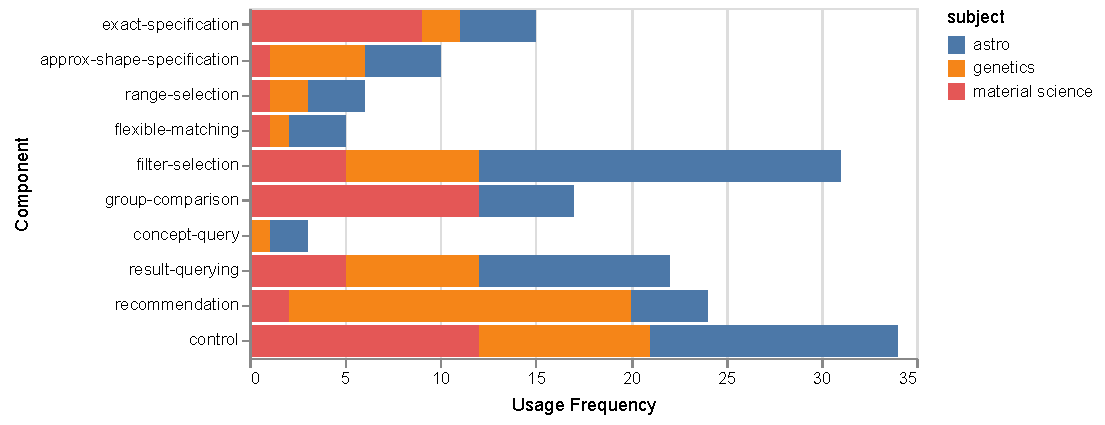
\includegraphics[width=\linewidth]{figures/usagefreqbysubject.pdf}
%   \caption{The number of times each component is used during the evaluation study, broken down by subject areas.}\label{fig:usagefreqbysubject}
% \end{figure}
\subsection{The Inefficiency of Sketching}
% \subsection{DC3: Closing the loop in VQS sense-making cycle with bottom-up data-driven inquries}
\par To our surprise, despite the prevalence of sketch-to-query systems in literature, Figure \ref{fig:feature_heatmap} shows that only two out of our nine users had a practical usage for querying by sketching. %Overall, bottom-up querying via drag-and-drop was more intuitive and more commonly used than top-down querying methods, such as sketching or input equations.
The main reason why participants did not find sketching useful was that they often do not start their analysis with a pattern in mind. Later, their intuition about what to query is derived from other visualizations that they see in the VQS, in which case it made more sense to query using those visualizations as examples directly. In addition, even if a user has a query pattern in mind, sketch queries can be ambiguous or even impossible to draw by sketching (e.g. A2 looked for a highly-varying signal enveloped by a sinusoidal pattern indicating planetary rotation 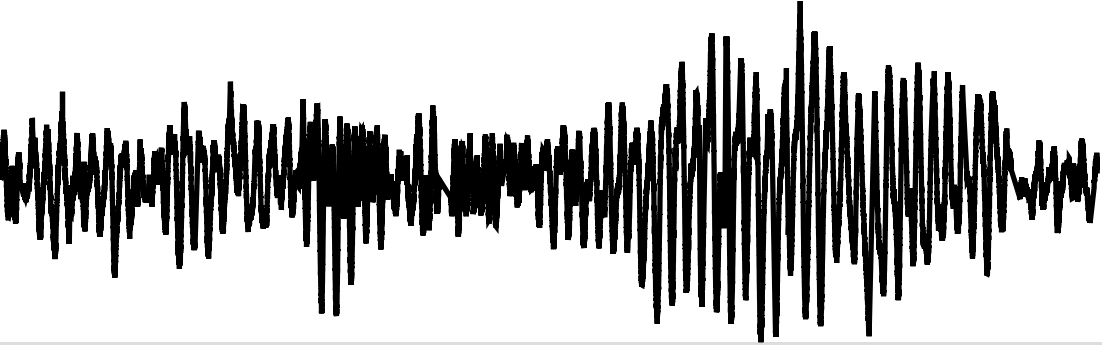
\includegraphics[width=2\baselineskip,keepaspectratio]{figures/impossible_sketch.png}).
\begin{figure}[h!]
  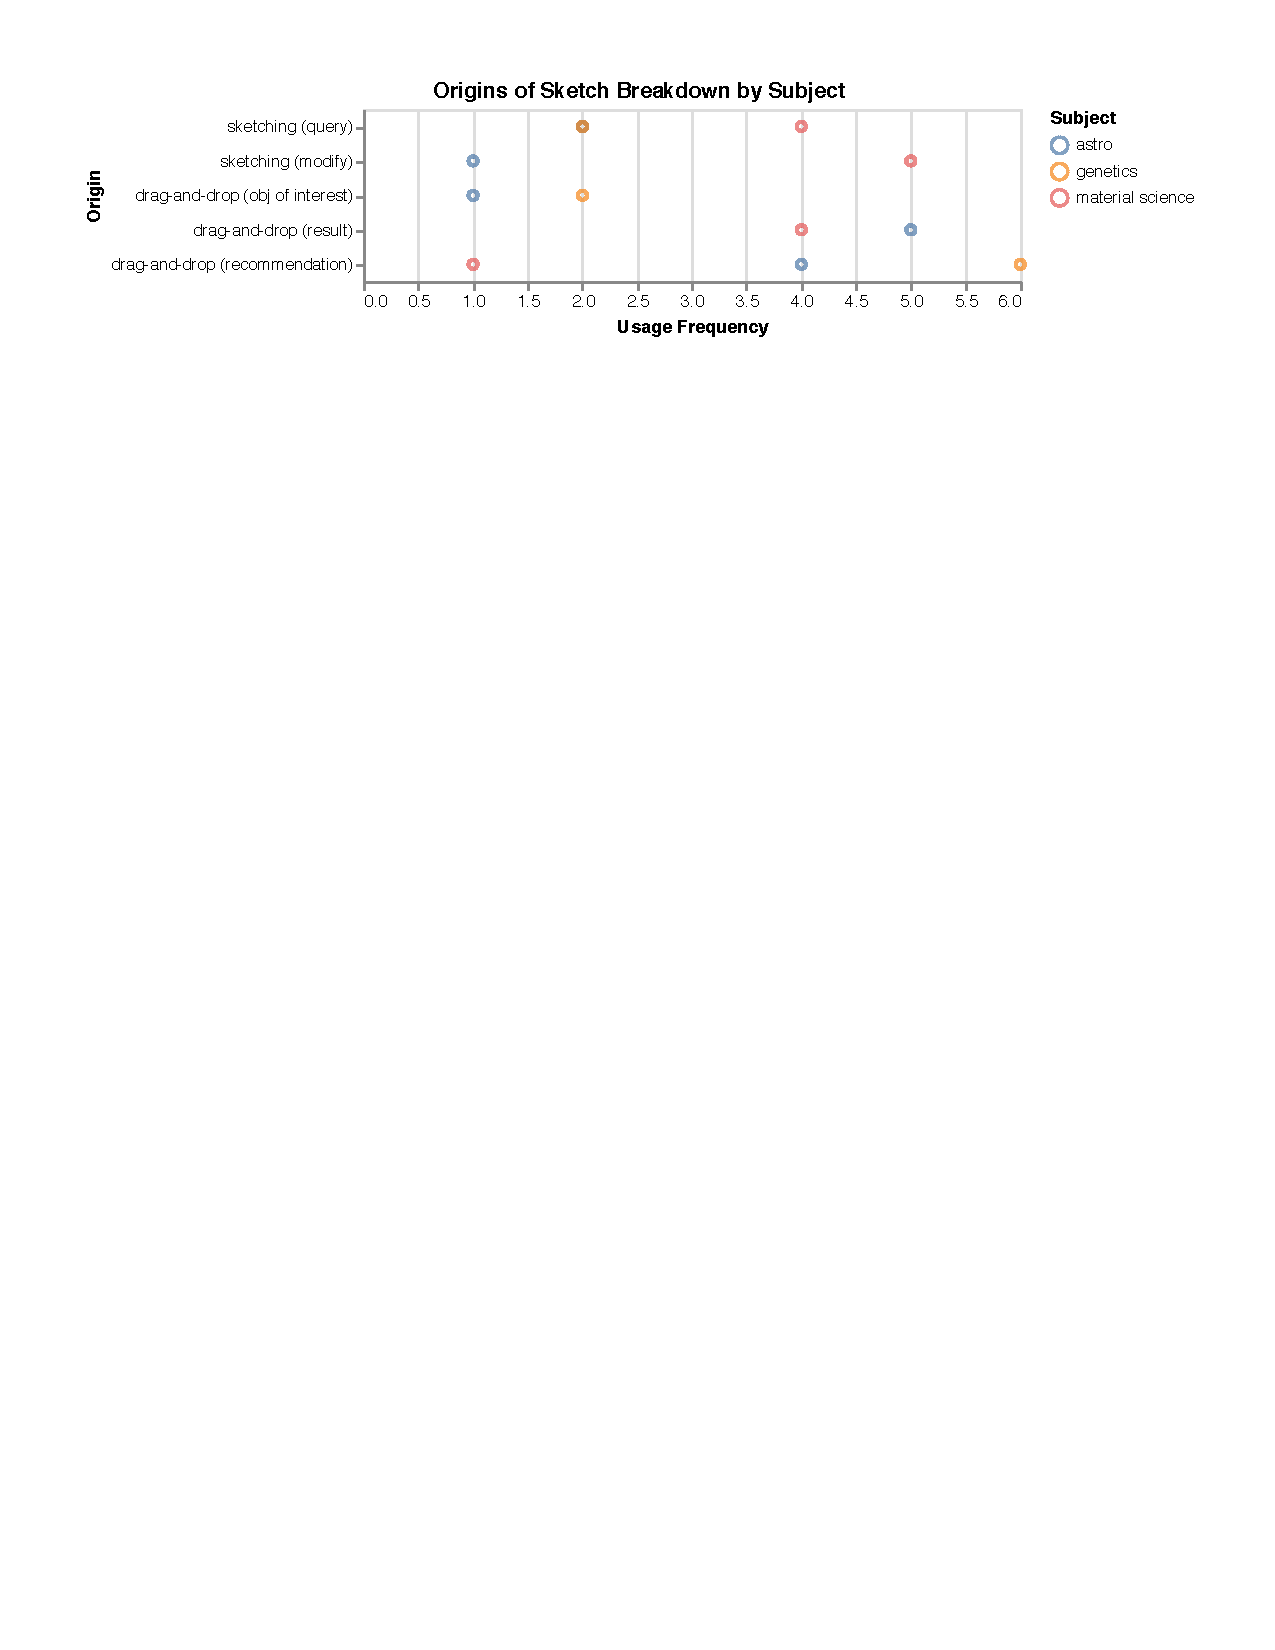
\includegraphics[width=\linewidth]{figures/origins_of_sketch_scatter.pdf}
  \caption{The number of times each sketch is generated by one of the workflows.}\label{fig:origins_of_sketch}
\end{figure}
\par Given these initial findings, we further investigate where the `sketch' (pattern on the canvas) originates. In particular, Figure~\ref{fig:origins_of_sketch} shows that pattern queries can originate from either drag-and-drop or sketching. Within these two types of actions, there can be different intentions behind the sketch. While all visualizations that could be drag-and-dropped must come from the result or recommendation pane, a query can come from a particular object that the participant is interested in or simply through peripheral browsing of visualization results, described in the next section. 
\par We note that there are many %\par The latter case is also supported by the 
unexpected use cases where sketching was simply used as a mechanism to modify an existing pattern query. For example, M2 first sketched a pattern to find solvent classes with anticorrelated properties without much success in returning a desired match.
%However, the sketched query did not return visualizations of interest.
So he instead dragged and dropped one of the peripheral visualizations that was close enough to his desired visualization and then smoothed out the noise due to outlier datapoints by tracing a sketch over the visualization, as shown in Figure \ref{query_modification} (left). M2 repeated this workflow twice in separate occurrences during the study and was able to derive insights from the results. Likewise, A3 was interested in pulsating stars that looked similar to stellar hotspots in terms of its dramatic amplitude fluctuations, but differ in that their patterns exhibited irregularities. Figure \ref{query_modification} (right) showed how she first picked out a regular pattern (suspected star spot), then modified it slightly so that the pattern looks more irregular.
%Likewise, A3 was interested in pulsating stars characterized by dramatic changes in the amplitudes of the light curves. During the search, hotspots on stellar surfaces often show up as false positives as they also result in dramatic amplitude fluctuations, but happen at a regular intervals. In the VQS, A3 looked for patterns that exhibits amplitude variations, but also some irregularities. As shown in Figure \ref{query_modification} (right), she first picked out a regular pattern (suspected star spot), then modified it slightly so that the pattern looks more irregular.
\begin{figure}[h!]
    \centering
    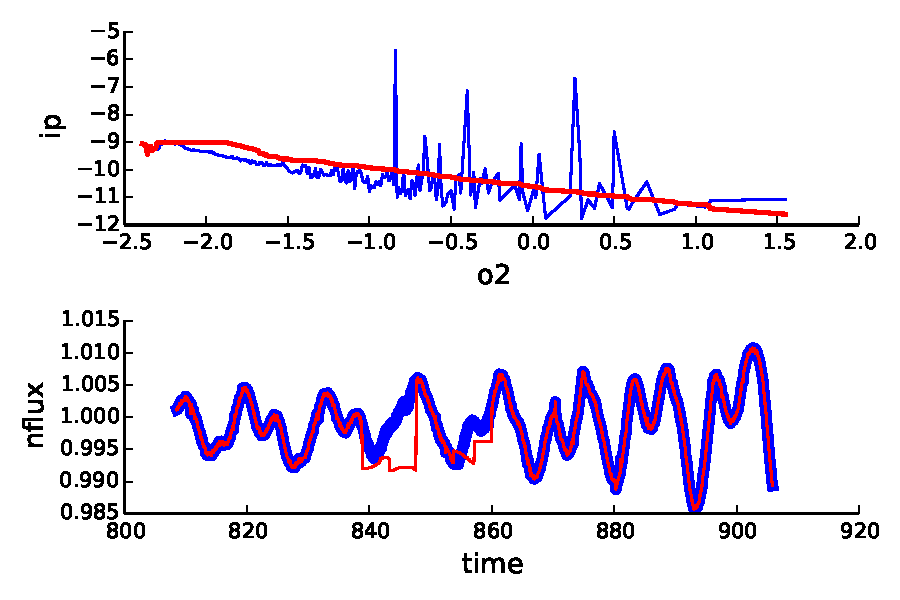
\includegraphics[width=\columnwidth]{figures/QueryModificationBySketch.pdf}
    \caption{\tvcg{Canvas traces from M2 (left) and A3 (right) during the study demonstrating query modification. The original drag-and-dropped query is shown in blue and the sketch-modified queries in red.}
    \label{query_modification}}
    \vspace{-10pt}
\end{figure}
\par The lack of practical use of top-down pattern specification is also reflected in the fact that none of the users queried by equation. In both astronomy and genetics use cases, the visualization patterns result from complex physical processes that could not be written down as an equation analytically. Even in the case of material science when analytical relationships do exist, it is challenging to formulate functional forms in an prescriptive, ad-hoc manner.
% Despite functional fitting being common in scientific data analysis, Figure \ref{feature_heatmap} shows that
% . However,
\par Both query by sketch and equations adopt a problematic assumption that analysts start with a known and easy-to-specify search pattern in mind. These findings suggest that while sketching is an useful analogy for people to express their queries, \emph{the existing ad-hoc, sketch-only model for visualization querying is insufficient without data examples that can help analysts jumpstart their exploration}. This finding has profound implications on the design of future VQSs, since Table~\ref{table:relatedwork} show that past work have primarily focused on optimizing the components in the top-down paradigm, without regards to how useful these features are in real-world analytic tasks.
%missing out largely on the key components in the other two paradigms \cut{(indicated by the absence of green features on the right hand side of the table)}.
We suspect that these limitation may be why existing sketch-to-query systems are not commonly adopted in practice. %This result points to a need for ----- in future VQSs. %This, however, points to an exciting direction for sketching interface in VQSs for developing advanced drawing and modification tools that enable more precise visualization query specification.} %ed coverage in addressing different types of analytics use cases
%For instance, material science discovered a known inverse relationship during e xploration
%Which is really interesting. Which is something that we observed experimentally also. That is an interesting insight right htere. This seems to suggest that there is a fundamental issue in if you want to try to get better on this axis, and get as low as possible, you lose out on the other axis.
%once they see it they know it but they don't know beforehand

\subsection{Practical Use of Bottom-up approaches}
\par \emph{Bottom-up data-driven inquiries are more common than top-down pattern specification when the users have no desired patterns in mind}, which is commonly the case for exploratory data analysis. This is highlighted by Figure~\ref{fig:feature_heatmap} which shows that top-down querying was only useful 29\% of the use cases, where as it was useful for 70\% of the use cases for bottom-up querying.
\par The prevalence of bottom-up approaches not only point to the need for result querying, but also providing recommendations for users without desired patterns in mind. As shown in Figure~\ref{fig:origins_of_sketch}, the most common use of result querying comes from querying via a visualization that lie in a cluster. Examples of how recommended trends can provoke further insightful actions comes from G2 and G3, who identified that the three representative patterns shown in \zv \cut{---induced genes (profiles with expression levels staying up), repressed genes (started high but went down), and transients (go up and then come down at different time points)---}corresponded to the same three groups of genes discussed in a recent publication\cite{Gloss2017}. The clusters provoked G2 to generate a hypothesis regarding the properties of transients: \textit{``Is that because all the transient groups get clustered together, can I get sharp patterns that rise and ebb at different time points?''} To verify this hypothesis, G2 increased the parameter controlling the number of clusters and noticed that the cluster no longer exhibited the clean, intuitive patterns he had seen earlier. G3 expressed a similar sentiment and proceeded by inspecting the visualizations in the cluster via drag-and-drop. He found a group of genes that all transitioned at the same timestep, while others transitioned at different timesteps. \cut{G3 described the process of using VQSs as doing ``detective work'' that provoked him to generate further scientific hypotheses as well as data actions.} 
%This includes inspecting the top-most similar visualizations that lie in the queried cluster. and finding visualizations that are similar to an object of interest that exhibits a desired pattern.
\par By browsing through the ranked list of result in \zv, participants were also able to gain a peripheral overview of the data and spot anomalies during exploration. For example, A1 spotted time series that were too faint to look like stars after applying the filter CLASS\_STAR=1. After browsing through a series query results and checking with an external database, he concluded that all stars have been incorrectly labelled with CLASS\_STAR=0 as 1 during data cleaning. 
\par Likewise, many participants envisioned use cases for pattern loading. The ability to load in data patterns as a query would enable users to compare visualizations between different experiments, species, or surveys, query with known patterns from an external reference catalog\techreport{ (e.g. important genes of interest, objects labeled as supernovae)}, or verify the results of a \techreport{simulation or }downstream analysis\techreport{ by finding similar patterns in their existing dataset}. The uploaded pattern also represents a more precise query specification that captures the desired features of a pattern \techreport{(e.g. amplitude, width of peak), }that cannot be precisely sketched. For example, the width of a supernovae light curve is characteristic to the radioactive decay rate of its chemical signature~\cite{Nugent1997}, so querying with an exact pattern template would be helpful for distinguishing the patterns of interest from noise.
 %We found that geneticists often gain their intuition about the data from the recommended representative trends. One example of rapid insight discovery

%the dataset had been incorrectly labelled with all the stars with CLASS\_STAR=0 as 1 during data cleaning.
\begin{figure}[h!]
  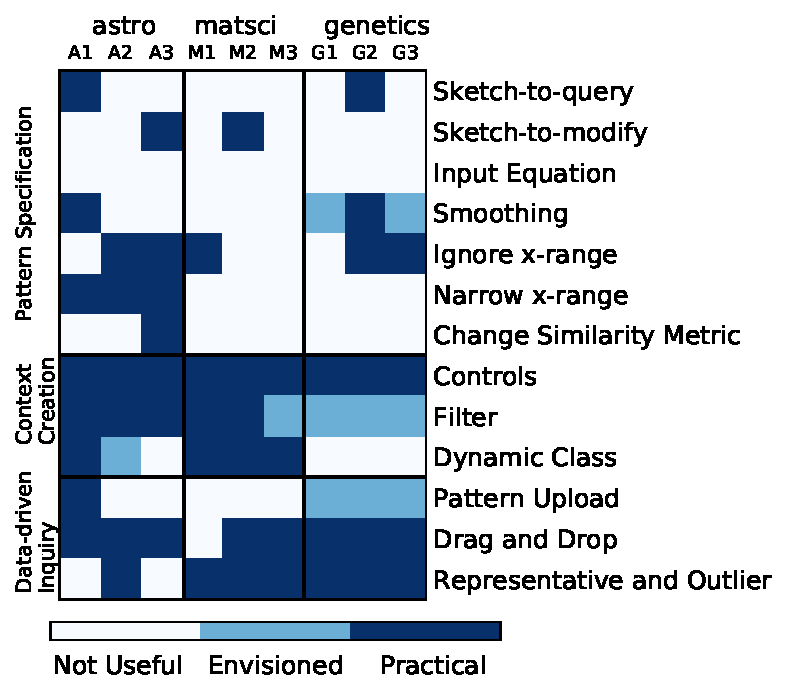
\includegraphics[width=0.8\linewidth]{figures/PENcoding.pdf}
  \caption{Heatmap of features categorized as practical usage, envisioned usage, and not useful. \techreport{We find that participants preferred to query using bottom-up methods such as drag-and-drop over top-down approaches such as sketching or input equations. Participants found that data faceting via filter constraints and dynamic class creation were powerful ways to compare between subgroups or filtered subsets. The columns are arranged in the order of subject areas and the features are arranged in the order of the three foraging acts.}}
  \label{fig:feature_heatmap}
\end{figure}
\subsection{Enriching Search with Context}
\par Past studies in taxonomies of visualization tasks have shown that it is important to design features that enable users to select relevant subsets of data in visual analytics~\cite{Amar2005,Heer2012}. %We designed two dynamic faceting features coupled with coordinated views that enabled users to specify subsets of data they are querying on and see immediate changes updated in the query, representative, and outlier results.
Figure~\ref{fig:feature_heatmap} shows that all participants either envisioned a use case or utilized features in the context creation paradigm to explore and compare subsets of their data.
\par A1 expressed that even though the filtering step could be easily done with an external tool and reloaded into \zv, filtering on-the-fly was a powerful way to dynamically test his hypothesis. Interactive filtering lowers the barrier between the iterative hypothesize-then-compare cycle during sensemaking, thereby enabling participants to test conditions and tune values that they would not have otherwise modified.
% echoing our previous finding that segmented workflow prevents extensive exploration.
During the study, participants used filtering to address questions such as: \textit{Are there more genes similar to a known activator when we subselect only the differentially expressed genes?} \techreport{\texttt{DIFFEXP=1} }(G2) or \textit{Can I find more supernovae candidates if I query only on objects that are bright and classified as a star?} \techreport{\texttt{flux\textgreater10 AND CLASS\_STAR=1} }(A1). Three participants had also used filtering as a way to pick out individual objects of interest to query with. For example, G2 set the filter as gene=9687 and explained that since ``this gene is regulated by the estrogen receptor, when we search for other genes that resemble this gene, we can find other genes that are potentially affected by the same factors.''
\par While filtering enabled users to narrow down to a selected data subset, dynamic class creation enabled users to compare relationships between multiple attributes and between subgroups of data. For example, M2 divided solvents in the database to eight different categories based on voltage properties, state of matter, and viscosity levels, by dynamically setting the cutoff values on the quantitative variables to create these classes. By exploring these custom classes, M2 learned that the relationship between viscosity and lithium solvation energy is independent of whether a solvent belongs to the class of high voltage or low voltage solvents and cited that dynamic class creation was central to learning about this previously-unknown attribute properties:
\begin{quote}
All this is really possible because of dynamic class creation, so this allows you to bucket your intuition and put that together. [...] I can now bucket things as high voltage stable, liquid stable, viscous, or not viscous and start doing this classification quickly and start to explore trends. [...] look how quickly we can do it!% Quite good!
\end{quote}
Context creation enables users to change the lens in which they look through when preforming visual querying, thereby creating more opportunities to see the queried data from different perspectives.
%Context creation is a useful ---- despite the --- pattern instance. Filtering still useful
%\par Participants employed \emph{a mix of bottom-up and top-down approaches when faceting through data in VQS}, including narrowing the search space based on some intuition about a phenomena, selecting individual visualizations, or specifying high-level groupings to compare and query with.
\newpage
\subsection{The Sensemaking Process in VQSs}
Given our observation on how analysts make use of each sensemaking process in practice, we further investigate how these sensemaking process interplay with each other dynamically in the context of an analysis workflow. 
% - Bottom up and context creation much more common than top-down. Stats \%. Brief Examples of each (How they are used in practice). 
% - BUT All three process are equally important. 
% - participants can go from one to the next and there is no single progression (e.g. context --> bottom -up --> top-down). 
% - Both the PageRank score (how important/“central” is the state is to the analysis?), raw occurrence of each state (how frequently is a feature categorized as part of the state used?) and the normalized self-directed edge score (how much user stays in that state?) coincide with what each subject area focuses on.

% We first examine the popularity of each sensemaking process based on how frequently they are used in the study. Figure~\ref{fig:feature_heatmap} show that features categorized as bottom-up (useful for 70\% of the use cases) and context creation (67\%) are much more useful compared top-down features (29\%). [Examples of Bottom up]. [Examples of Context Creation]. 
%Despite differing in levels of usage, each sensemaking process fulfills a central role in participants' analysis. 
\par Figure~\ref{fig:transition} illustrates the state transitions computed based on event sequences from the evaluation study. Each event sequence is separated by labeled session breaks signaling the beginning of a new line of inquiry. The edges denote the probability that an analyst in the particular subject area will go from one sensemaking process to the next. Self-direct edges indicate the probability that the analyst would stay in the same state. The transition model exemplifies how participants adopted a diverse set of workflows based on the unique set of research questions they brought to the study. We learn that the three sensemaking process does not simply follow a linear progression, going from unknown to known pattern instance and visualized attributes. Instead, the high connectivity of the transition model illustrates how these three equally-important processes form a sensemaking loop. The VQS sensemaking loop represents iterative acts of dynamic foraging and hypothesis generation. This flexibility is enabled by the diverse set of potential workflows that could be constructed for addressing a wide range of analytical inquiries.%single-directional 

\begin{figure}[h!]
  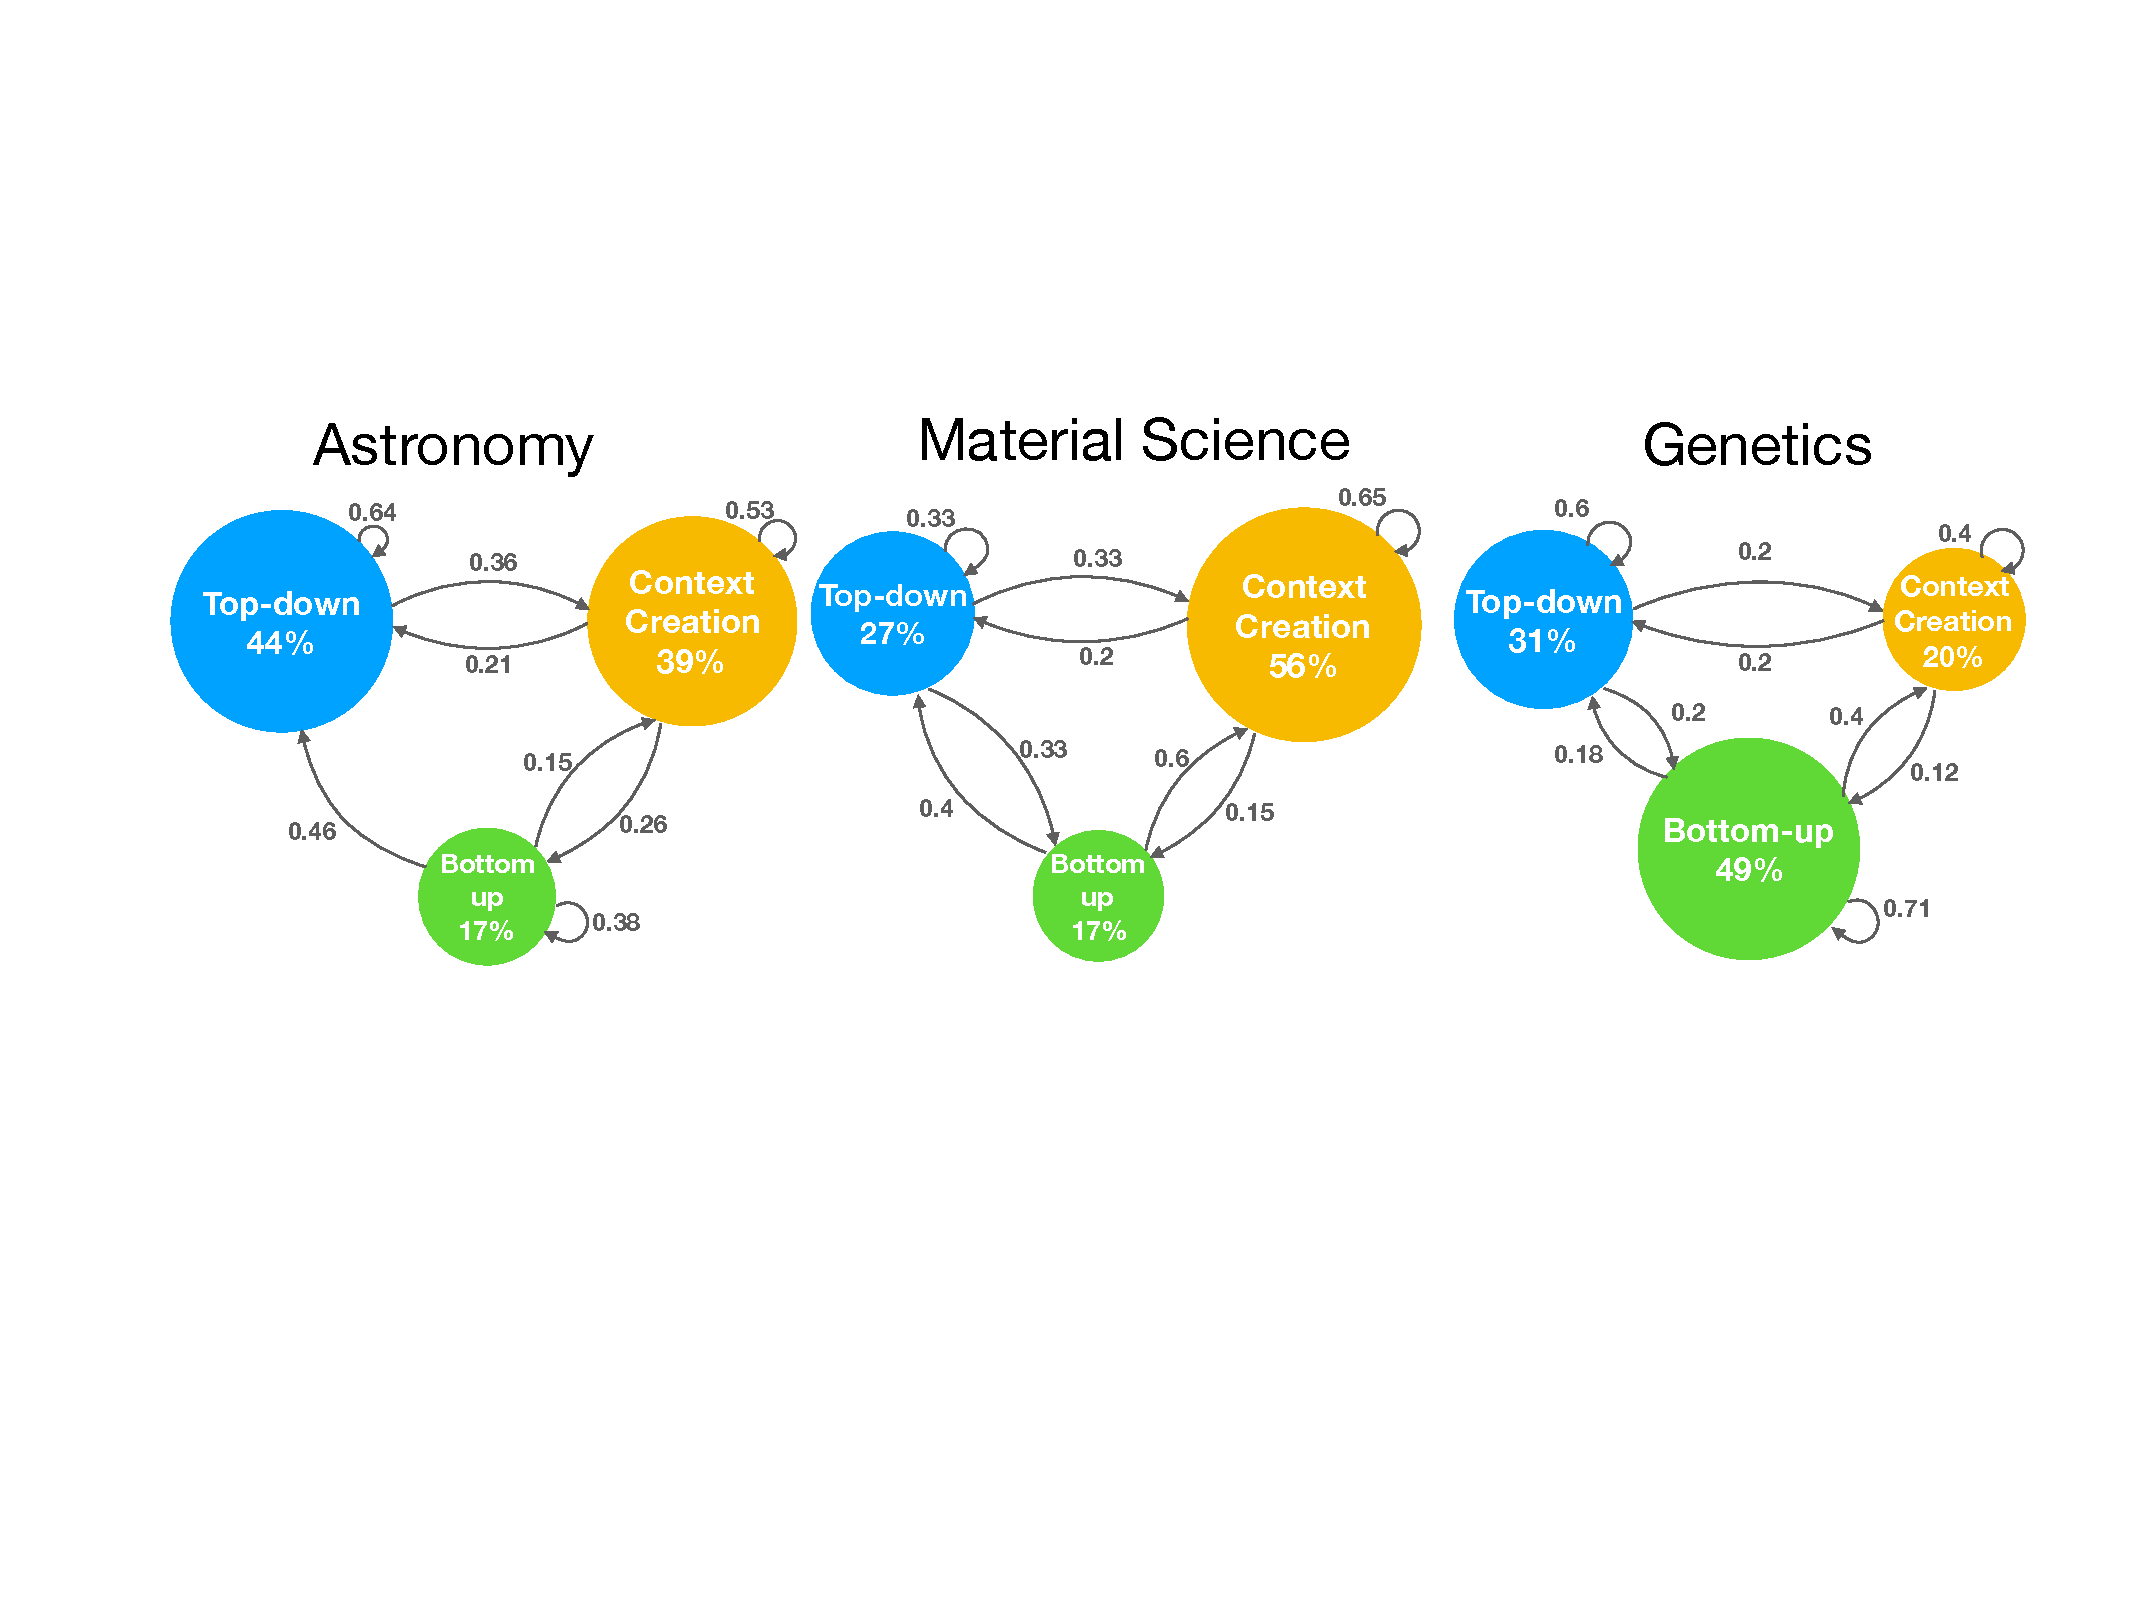
\includegraphics[width=\linewidth]{figures/transition.pdf}
  \caption{Markov model computed based on evaluation study event sequences illustrating how analysts move between different sensemaking processes. Nodes are scaled according to the eigenvector centrality, which represents the percentage of time users spend in a particular state.}\label{fig:transition}
\end{figure}
% Similar to the sensemaking model proposed by Pirolli and Card~\cite{Pirolli}, the ---- sensemaking loop representing iterative process 
% ---- highlights how the two newly discovered VQS sensemaking process in this paper are essential for `closing the loop' between the sensemaking acts in VQSs. %, equally important  
% both the browsing-act through recommendations and performing search via these results are 
%These examples show that both the browsing-act through recommendations and performing search via these results are 
%The three sensemaking ----- not mutually exclusive, participants can go from one to the next and there is no single progression (e.g. context --> bottom -up --> top-down). Iterative blah blah. three process are equally important. 
%The three paradigms of sensemaking described earlier are not mutually exclusive. 
%Different sensemaking processes can be useful for different problem contexts.  
\par To study how important each sensemaking process is for participant's overall analysis, we compute the eigenvector centrality of each graph, displayed as node labels in Figure~\ref{fig:transition}. These values represent the percentage of time users would spend in each of the sensemaking process when the transition model has evolved to a steady state. We find that participants often construct a central workflow around a main sensemaking process and interleave variations with the two other processes as they iterate on the analytic task. The central paradigm adopted by each use case is tightly coupled with characteristics of the analytic challenges presented by each subject area. For example, astronomers focused largely on performing top-down pattern specification, while filtering on the visualization space. Material scientists adopt focuses more heavily on the context creation through dynamic classes than top-down pattern specification. Geneticists relied heavily on bottom-up querying through recommendations to jumpstart their queries. Despite the differing levels of usage from each subject area, we learn that \textit{each sensemaking process fulfills a central role in participants' analysis to address their high-level research objectives}. 